\documentclass{article}


\usepackage{arxiv}

\usepackage[utf8]{inputenc} % allow utf-8 input
\usepackage[T1]{fontenc}    % use 8-bit T1 fonts
\usepackage{hyperref}       % hyperlinks
\usepackage{url}            % simple URL typesetting
\usepackage{booktabs}       % professional-quality tables
\usepackage{amsfonts}       % blackboard math symbols
\usepackage{nicefrac}       % compact symbols for 1/2, etc.
\usepackage{microtype}      % microtypography
\usepackage{lipsum}
\usepackage{graphicx}
\usepackage[russian]{babel}
\usepackage{layout}
\usepackage{amsmath}
\usepackage{booktabs}
\usepackage{array}
\newcolumntype{L}{>{\centering\arraybackslash}m{3cm}}
\newcolumntype{P}[1]{>{\centering\arraybackslash}p{#1}}

\graphicspath{{rcs/}}

\title{Построение индекса сентиментов для анализа рынка акций}

\author{
  Бучко Даниил Владимирович \\
  Факультет Экономических Наук\\
  Студент, 3-ий курс бакалавриата \\
  НИУ ВШЭ, г. Москва\\
  \texttt{dvbuchko@edu.hse.ru} \\
  %% examples of more authors
   \And
 Соколова Татьяна Владимировна \\
  Факультет Экономических Наук \\
  Старший преподаватель \\
  Базовая кафедра инфраструктуры финансовых рынков \\
  Аналитик в ЛАФР, НИУ ВШЭ, г. Москва \\
  \texttt{tv.sokolova@hse.ru} \\
  %% \AND
  %% Coauthor \\
  %% Affiliation \\
  %% Address \\
  %% \texttt{email} \\
  %% \And
  %% Coauthor \\
  %% Affiliation \\
  %% Address \\
  %% \texttt{email} \\
  %% \And
  %% Coauthor \\
  %% Affiliation \\
  %% Address \\
  %% \texttt{email} \\
}

\begin{document}
\maketitle

\begin{abstract}

Когда заинтересованный исследователь попадает на финансовый рынок, для него открывается множество инструментов для принятся инвестиционных решений. Все эти инструменты в основе своей базируются на двух основновополагающих источниках: на фундаментальной и технической информации. Использование данных из этих источников подразумевает не только первичную обработку, но и последующую интерпертацию полученных результатов, что является достаточно трудозатратным процессом. А что если есть иные источники информации, которые могут передавать содержательный смысл анализа общедоступных данных? Что если направлять усилия не на исследования состояния определенной компании, а попробовать прислушаться к тому, что говорят люди об этой компании? Может быть у нас получится получить общее представление о состоянии компании, основываясь на разрозненные мнения? В данном исследовании я проведу анализ альтернативных источников принятия решений и проверю их эффективность на примере российского рынка акций. В качестве таких источников будут выступать финансовые форумы.


\end{abstract}


% keywords can be removed
% \keywords{First keyword \and Second keyword \and More}


\section*{Вступление}
Я бы хотел провести читателя этой статьи по пути вопросов и ответов, которые возникают сами собой в ходе решения любой поставленной задачи. Поэтому, сформулируем первый логичный вопрос: 
<<\emph{Что мы хотим сделать?}>>. Как было сказано раннее в асбстракте, мы бы хотели получить полезную информацию о компаниях, торгующих ценными бумагами, не прибегая к трудозатратным операциям, предполагающим знания финансовой отчетности или технического анализа. Следующий логичный вопрос: <<Что это за информация и почему её можно считать ценной?>> Частично на этот вопрос мы ответим в главе \ref{sec:data}, где планируется выбрать данные и определиться с их источниками, а частично $-$ в главе \ref{sec:portfolio}, где определимся с тем, насколько ценной оказалась полученная информация. В главе  \ref{sec:data} я также рассмотрю особенности и способы получения данных. Будет показано на примерах, как выглядит структура источников, каким образом осуществляется автоматический сбор и обработка данных. Затем полученные данные мы начнем активно исследовать в главе  \ref{sec:prepare}, чтобы ответить на следующий вопрос: <<Как использовать полученные данные?>> При подробном расммотрении я опишу основные тонкости и механизмы предобработки полученных текстов, покажу особенности конкретно наших данных, посчитаю статистики и визуализирую основные результаты. В главе \ref{sec:model} мы займемся вопросами непосредственного моделирования языка при помощи машинного обучения и нейронных сетей: сформулируем задачу, выберем метрики, а затем подберем подходящую модель. В заключительной главе \ref{sec:conclusion} мы подведем итоги исследования.

\section{Аналогичные исследования}

Перед тем как перейти к рассмотрению полученных результатов, прокомментируем уже произведенные исследования в рассматриваемой области. Первым делом хочется отметить работу Van-Dai Ta (2020), в которой авторы построили систему оптимизации портфеля, основанную на предсказаниях котировок ценных бумаг. Принимая на вход данные по историческим значениям доходностей, авторы не только устанавливали закономерности в данных,  но и формировали оптимальные портфели ценных бумаг. В результате исследования были сформированы высокодоходные активы, в разы опережающие бэнчмарки по доходности. 
\par В работе Birbeck and Cliff (2018) был использован анализ сентмента, но с очень интересной особенностью: текстовые сообщения размечались не по принципу значения слов, а по принципу изменения цены для конкретно рассматриваемой ценной бумаги. К примеру, если за указанный час акции теслы росли, то любые обсуждения за этот же час можно считать сигналами к покупке и наоборот. Удивительные возможности данного подхода заключаются в том, что количество используемых данных ограничивается лишь количичеством сообщений в социальных сетях, а сам процесс разметки полностью автоматизирован и  не представляет сложностей. Данный подход позволил авторам получить месячную доходность в размере 5.18\%, при совершении 468 сделок.
\par Наиболее близкий подход к нашему исследованию был предложен группой исследователей\footnote{Paolo Cremonesi, Chiara Francalanci, Alessandro Poli, Roberto Pagano, Luca Mazzoni, Alberto Maggioni, Mehdi Elahi (2018)}. Авторы таким же образом исследовали сообщения с твиттера, разделяя их на 3 различных группы: положительные, нейтральные и негативные, но использовали полученные данные для предсказания котировок в краткосрочных сделках. Авторы пришли к выводу, что сентименты компаний заслуживают право называться фундаментальными переменными.
\par Из вышеописанных статей можно сделать вывод о том, что исследованиями в области применения нейронных сетей в финансах, в частности оценкой влияния человеческого мнения на рынок акций, занимаются множество людей и актуальность этой темы до сих пор не поддается сомнениям.


\section{Получение данных.}
\label{sec:data}



\subsection*{Какие данные использовать?}

Информацию об окружающем мире можно черпать из различных источников. Очевидно, что любой источник информационного потока имеет свои особенности и отличительные черты. К примеру, информация, публикуемая в журналах, обычно проходит через долгие корректировки, и к моменту выпуска издания, она может частично или полностью искажаться, утрачивать свою значимость и актуальность, в зависимости от задачи, в которой эта информация планировалась использоваться. Аналогичными свойствами можно охарактеризовать информацию, получаемую из новостей, регулярных аналитических сводок и стриминговых сервисов. Более того, важной отличительной чертой всех этих источников является то, что информация, получаемая на выходе, проходит через множество рук и любые конкурентные приемущества связанные с ценностью новой информации могут быть утеряны, потому что всегда будет некий посредник между исследователем и событиями.  
\par Поэтому, для нашей задачи,$-$ оперативно получать потенциально полезную информацию о финансовом рынке $-$ необходимо выбрать источники, обладающие подходящими свойствами:

\begin{enumerate}
	\item Релевантность. Важнее всего, чтобы информация с нашего источника имела отношение к ценным бумагам и гипотетически имела предсказательную силу. Ведь именно для этого мы и собираемся её собирать и обрабатывать. Отсекаем любые неэкономические источники данных.
	\item Доступность. Это свойство позволит оперативно получать факты об изменениях на рынке без дополнительных ограничений, накладываемых посредниками или высокими издержками.  Исключаем источники данных, за которые необходимо платить. 
	\item Высокая частотность данных. Очень удобно выбирать такой источник, информация с которого была бы в достаточном количестве, для проведения простейшего статистистического анализа. Кроме этого, это свойство дает возможность моментально адаптироваться к любым шокам, меняющим конъюктуру рынка ценных бумаг. Концентрируемся на постоянно обновляющихся, высокочастотных источниках данных.
\end{enumerate}
Учитывая все аспекты, приведенные выше, я решил остановиться на текстовых источниках данных. Релевантность кокретизируется в текстовых данных, описывающих ситуацию на рынке акций. Как быть с доступностью? Здесь можно выбрать источники, не требующие денежных и временных издержек на ожидание получения информации $-$ финансовые форумы и группы в социальных сетях. Заметим, что такие источники удовлетворяют и последнему свойству $-$ свойству высокой частотности. Многие онлайн-платформы, ставшие привычным местом для обсуждения инвестиционных идей и стратегий существуют на российском рынке аж с конца 2000-х годов и активно развиваются по сей день.

\subsection{Интернет сообщества: сайты}

Безусловным лидером на на российском рынке финансовой информации является интернет платформа \href{www.mfd.ru}{MFD}. Судя по информации об интернет-ресурсе\footnote{https://mfd.ru/about/}, эта платформа работает с $1996$ года и объединяет ежедневно более $10000$ человек.
Вторым кандидатом на подходящий источник информации является интернет сообщество \href{https://smart-lab.ru}{Smart-Lab}. Помимо указанных ресурсов, существует несколько интересных организаций, предоставляющих финансовую информацию, среди них: \href{http://cbonds.ru}{Cbonds}, \href{https://quote.rbc.ru}{Quote РБК}, \href{https://investfunds.ru}{InvestFunds}. 
Единственное отличие последних состоит в том, что они работают по принципу предоставления контента, а значит не до конца удовлетворяют нашей предпосылке о доступности. Остановимся на MFD.

\subsection{Интернет сообщества: телеграм каналы}
Телеграм-каналы стали популярны на пике введения блокировок в результате отказа основателя компании от предоставления ключей шифрования государству\footnote{https://www.sostav.ru/publication/telegram-38688.html}. Сложно судить, что стало ключевым фактором в успехе телеграма, будь то зажигающая идея противостояния государству, которую так любит молодежь, либо удобный интерфейс, но телеграм полюбили и не обошли стороной люди, имеющие непосредственное отношение к финансовым рынкам. Так или иначе, телеграм предоставляет удобный и простой способ обсуждения различных тематик, поэтому заприметим этот источник информации как задел на будущие исследования и вернемся к его обсуждению в заключительной секции этого исследования. 
\par Итак, мы разобрались с тем, что интернет площадка MFD обладает всеми необходимыми для нашего исследования характеристиками. Следующий вопрос: <<Какую конкретно информацию, мы собираемся использовать?>>. Существуют многочисленные исследования в области анализа влияния текстовой информации на изменение в доходности ценных бумаг\footnote{Работы [1], [2], [3] в списке литературы}. В данных исследованиях проверялась гипотеза о влиянии социальных сетей на доходность акций и индексов. Более того, были предприняты успешные попытки построить регрессионные модели, объясняющие доходность индексов, ориентируясь только на сентименты сообщений в социальных сетях. Попробуем сделать подобное исследование, но с использованием более современного подхода в области моделирования языка и на российском рынке акций.

\subsection{Сбор информации с интернет-ресурсов}
Поскольку мы определились с тем, что и откуда будем собирать, настало время понять, каким образом выполнить эту задачу. Для этого нужно получить представление о строении сайтов и понять, из каких деталей состоят веб-страницы. Ниже можно видеть переписку участников финансового форума в той форме, в которой её видит человек и в том обличии, в каком она предстает перед браузером. 
\begin{figure}[h]
	\center{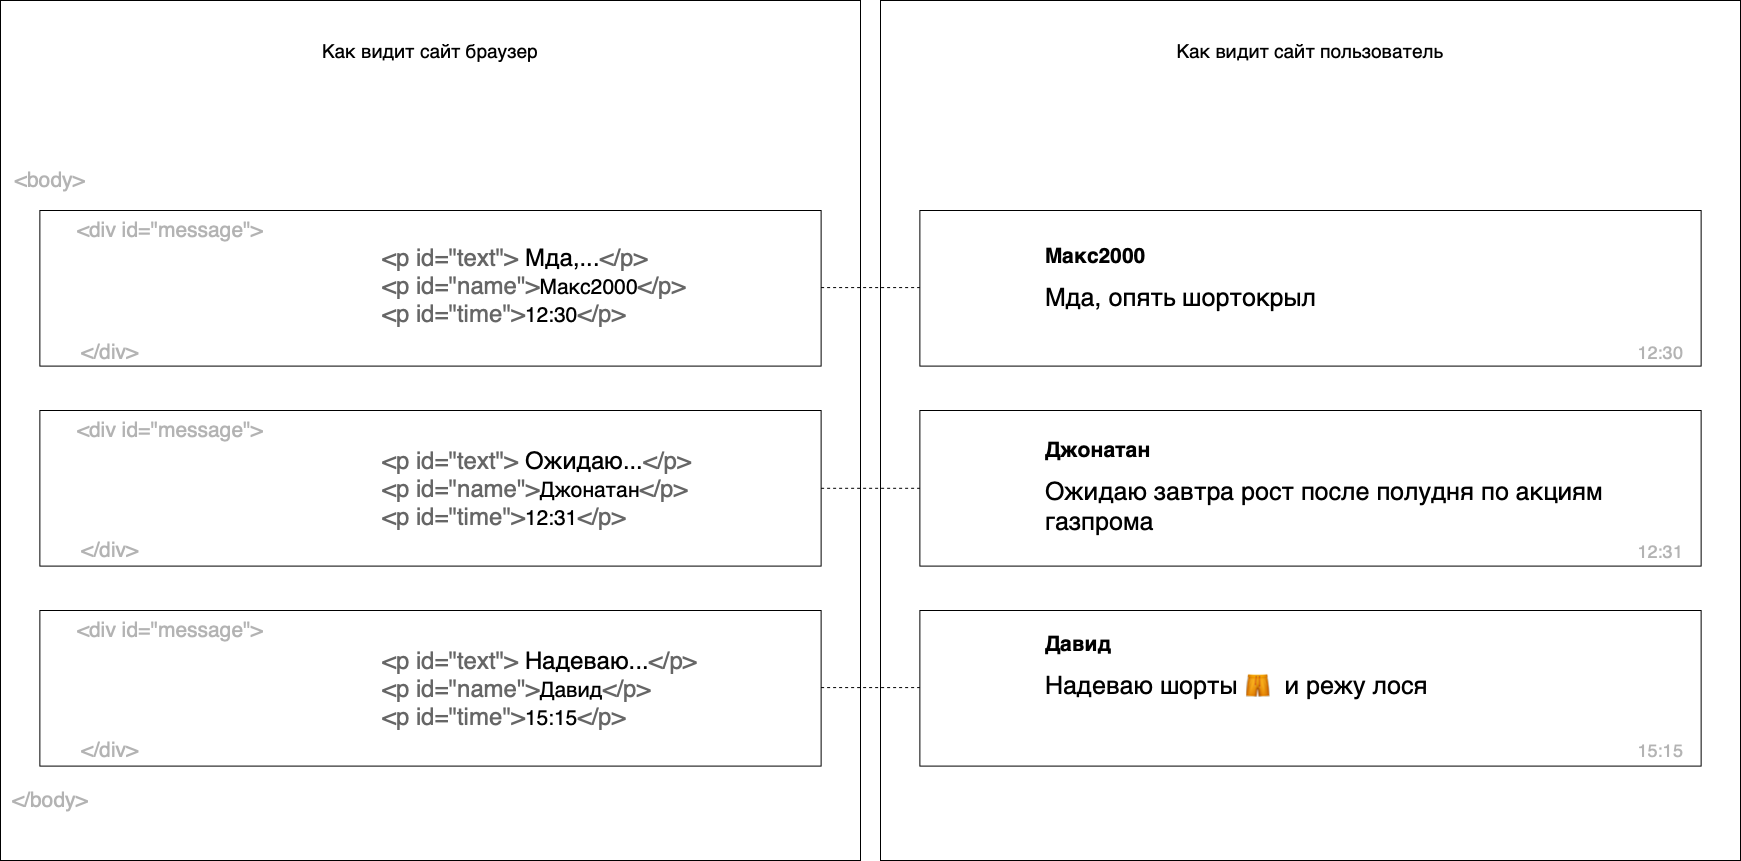
\includegraphics[scale=0.27]{html.png}}
	\caption{Каким образом информация предоставлена на сайте}
	\label{fig:image}
\end{figure} \\
Заметим, что каждое сообщение находится в соответствующем блоке (контейнере). Таким блокам присваивается метка <<message>>, явно указывающая на содержимое контейнера. Весь процесс сбора данных состоит в том, чтобы отыскать все контейнеры на странице, получить их содержимое и перейти к следующей странице. Обратим внимание на то, как хорошо структурирована информация на этом примере. В реальности сайты редко бывают статическими, обычно они меняют свою структуру под воздействием пользовательский действий. Но это явно не случай российских форумов, написанных с конца 90-х годов. Кроме того, нужно с осторожностью пользоваться автоматическим сбором данных. Некоторые сайты запрещают использование парсеров, потому что слишком частые запросы страниц нагружают сервера и неправильно написанный код может значительно затруднить пропускную способность интернет-ресурса. Переходим к следующему шагу. \\

\begin{table}[h]
	\caption{Примеры полученных сообщений}
	\centering
	\begin{tabular}{llp{9.45cm}l}
		\toprule
		Дата сообщения     &  Имя пользователя    & Текст сообщения  \\
		\midrule
		09.11.2014 15:46     & Веном  & ШОРТИТЕ!!!		\\
		09.11.2014 17:17     & михаил2 & ты первый	      \\
		09.11.2014 17:43     & петрович       & Так вы будете бить рекорд погружения или как?  \\
		09.11.2014 18:09     & Веном  & Рубль непоколебим в России.  Доллар растёт		\\
		09.11.2014 18:27     & capitan & Начинайте	мне еще пару тысяч прикупить надо...	      \\
		10.11.2014 14:33     & capitan       & Прикупил себе PLZL.  \\
		10.11.2014 15:47     & capitan       & Главное не слейся раньше времени	как на Алросе) хотя я и сам так сделал)  \\
		10.11.2014 16:37   & драконорожденный       & Не	не сольюсь.    А с Алросой я ошибку сделал. Надо было смотреть на то \\    
		11.11.2014 11:36     & драконорожденный       & Думаю	что эту цену мы увидим не раньше следующей весны...Я предупреждал \\    
		
		14.11.2014 22:52   & МарКс       & Все после таких новостей понятно стало \\    
		15.11.2014 22:59     & трейдерсрублевки       & http://oilru.com/news/436599/	 \\    
		\bottomrule
	\end{tabular}
	\label{tab:table}
\end{table}

\section{Подготовка данных}
\label{sec:prepare}
В результате сбора данных были получены сообщения с 2008 по 2020 год по компаниям из разных групп капитализаций: маленькие, средние и большие. (см. примеры Таблица \ref{tab:table}). Перед тем, как перейти к процессу построения моделей, необходимо предобработать текст таким образом, чтобы максимально исключить всю лишнюю информацию. Для этого текст, при помощи регулярных выражений, очищается от любой пунктуации, любых небуквенных символов, лишних пробелов и неинформативных ссылок и слов. После этого, каждое предложение приводится к нижнему регистру, лемматизируется (то есть приводится к своей начальной форме) и стеммингуется (обрезается таким образом, чтобы от слова осталась только его основа). Произведенные операции позволяют сократить количество неиформативных признаков, тем самым улучшая скорость и точность работы оптимизационных алгоритмов. В результате подобной обработки, сообщения стали иметь следующий вид:

\begin{table}[h]
	\caption{Сообщения после обработки}
	\centering
	\begin{tabular}{llp{9.45cm}l}
		\toprule
		Дата сообщения     &  Имя пользователя    & Текст сообщения  \\
		\midrule
		09.11.2014 15:46     & Веном  & шорт		\\
		09.11.2014 17:17     & михаил2 & ты	перв    \\
		09.11.2014 17:43     & петрович       &  так вы быт бит рекорд погружен ил как   \\
		09.11.2014 18:09     & Веном  & рубл непоколебим в росс доллар раст	\\
		09.11.2014 18:27     & capitan & начина я ещ пар тысяч прикупа	      \\
		10.11.2014 14:33     & capitan       & прикупа себ plzl  \\
		10.11.2014 15:47     & capitan       & главн не слива ран врем как на алрос хот я и сам так сдела  \\
		10.11.2014 16:37   & драконорожденный       & не не слива а с алрос я ошибк сдела быт смотрет на то \\    
		11.11.2014 11:36     & драконорожденный       & дума что этот цен мы увидет не ран след весн я предупрежда \\    
		
		14.11.2014 22:52   & МарКс       &  посл так новост понятн станов \\    
		15.11.2014 22:59     & трейдерсрублевки       &  	 \\    
		\bottomrule
	\end{tabular}
	\label{tab:table2}
\end{table}

Обратим внимание на то, что сообщения в большинстве случаев не потеряли свой основной смысл, однако количество уникальных слов сократилось в 4 раза: с $131,530$ до $34,733$. Такой подход в обаботке текстов имеет свои ограничения, и иногда останавливаются на этапе лемматизации, но как мы увидим далее, именно такой способ подготовки сообщений позволит делать наиболее точные прогнозы в рамках конкретно нашей задачи. В приложении можно посмотреть на другие интересные статистики по датасету (см. Главу \ref{chap:additional}).

\begin{figure}[h]
	\centering
	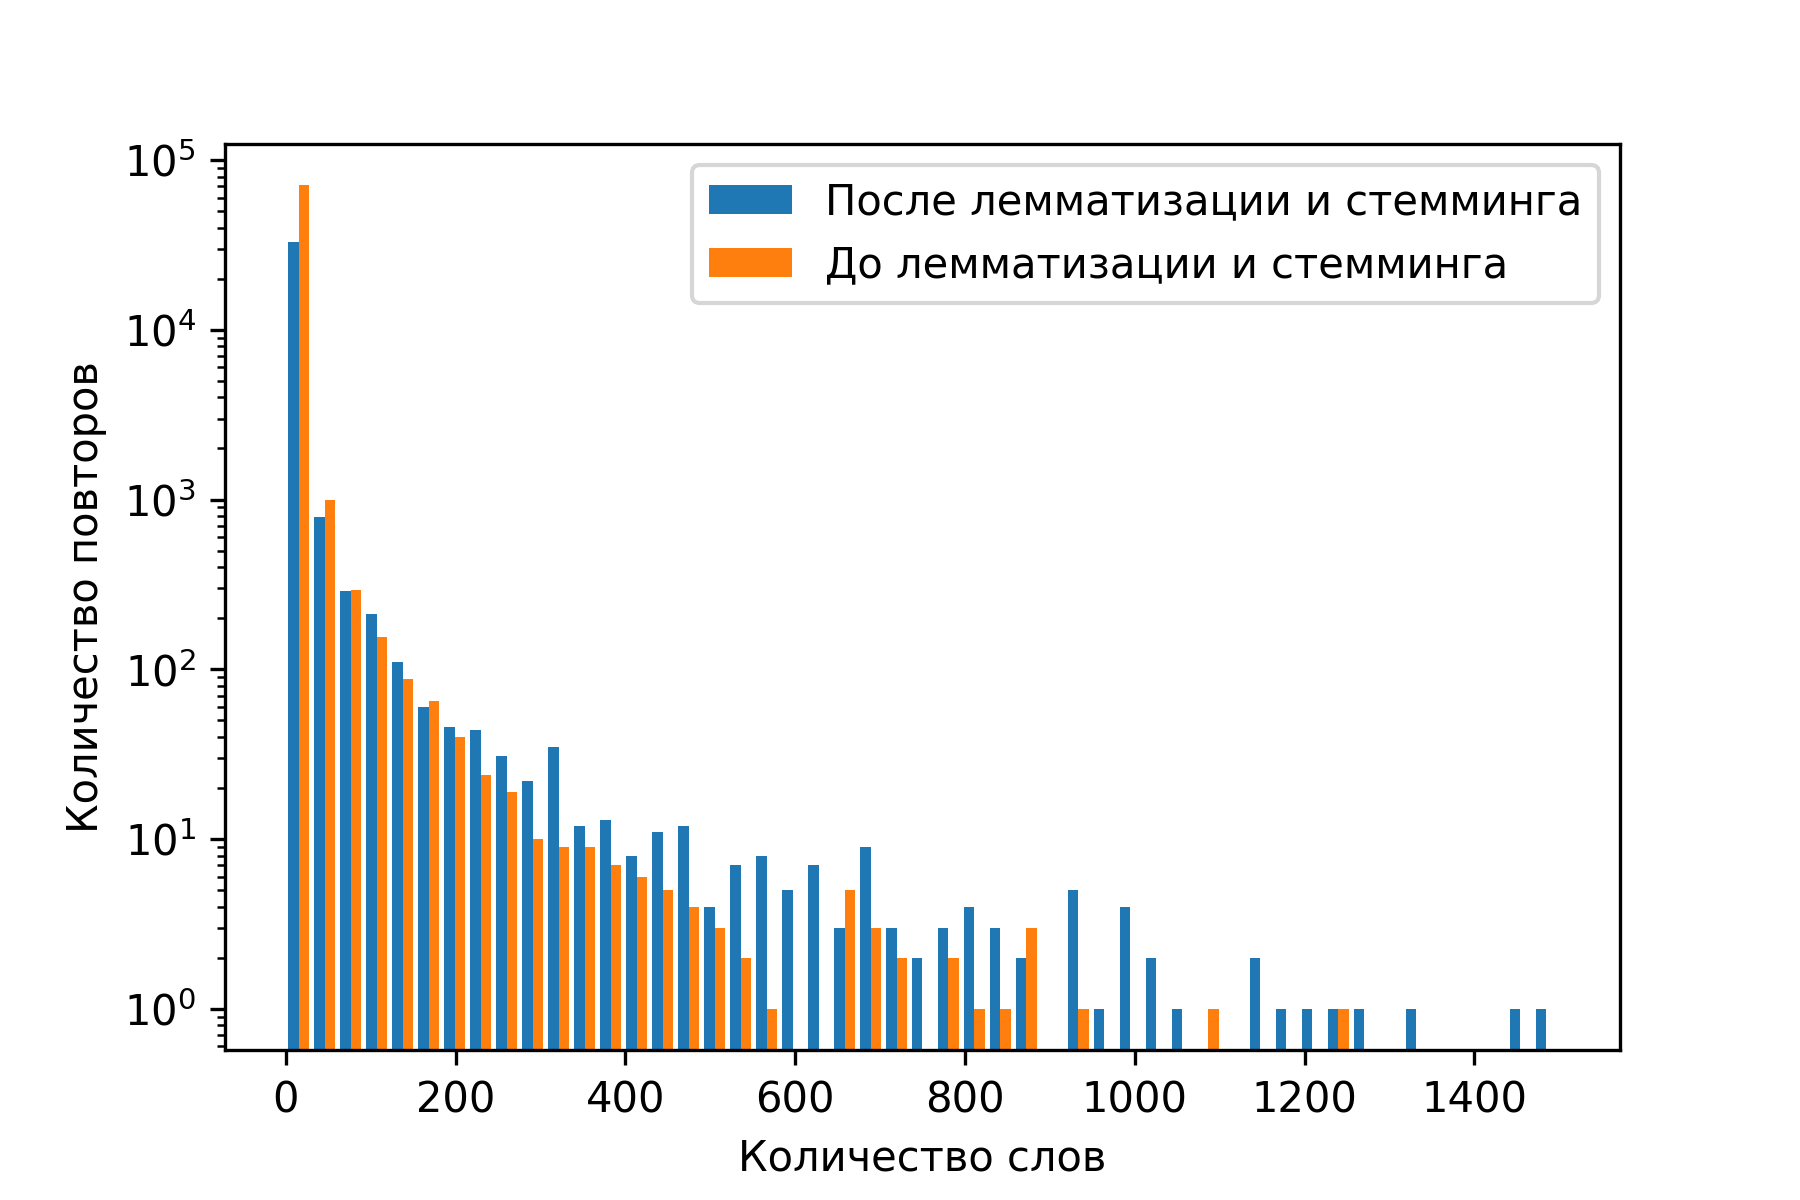
\includegraphics[scale=0.65]{before_after.png}
	\caption{Распределение слов в тренировочном наборе данных}
	\label{pic:dist}
\end{figure}

Как можно видеть из рисунка \ref{pic:dist}, в результате обработки данных частотность слов распредилилась более равномерно, уменьшая долю выбросов в выборке. На изображение не попали слова с очень низкой частотностью, для сохранения наглядности. В приложении есть таблица \ref{tab:table4}, показывающая примеры частоупотребляемых и редкоупотребляемых слов. Переходим к выбору модели.

\section{Выбор модели}
\label{sec:model}
Следующий момент, который мы должны для себя решить $-$ как использовать собранные данные? В работах \cite{2014oli}, \cite{2017ren} авторы предпринимали попытки объяснить доходность бумаг, исходя из гипотезы, которую можно сформулировать следующим образом: <<Эмоциональный фон, складывающийся вокруг определенной бумаги, влияет на решение инвестора (по крайней мере частного) о покупке или продаже той или иной бумаги>>. Для того чтобы проверить эту гипотезу, нам необходимо построить модель $F(.)$, которая бы переводила сообщения во множество эмоциональных признаков по следующей схеме:

\begin{equation}
\label{eq:F}
F(\text{сообщение}) = 
\begin{cases}
3, &\text{если сообщение носит позитивный окрас}\\
2, &\text{если сообщение не относится к финансовому рынку} \\
1, &\text{если сообщение носит негативный эмоциональный окрас} \\
\end{cases}
\end{equation}

Получается, что для нас, как для исследователей, задача сводится к построению модели, разделяющей все сообщения на 3 группы. С точки зрения машинного обучения, такая задача именуется задачей классификации. Выделим ключевые особенности нашего набора данных, чтобы выбрать подходящую модель:

\begin{enumerate}
	\item Изменчивость лексики во времени. Некоторые фразы, под влиянием различных культурных особенностей, меняют со временем то, как мы выражаем свои мысли, поэтому из всего количества собранных данных, для обучения были взяты сообщения из различных временных промежутков.
	\item Постобработанные данные не имеют меток класса. Простым языком, чтобы использовать алгоритмы обучения с учителем, нам необходимо дополнительно вручную разметить данные. Особенности рутинной ручной разметки ограничивают количество данных для обучения, поэтому из этого пункта возникает следующая характерная черта.
	\item Относительно небольшой датасет. В результате разметки совместными усилиями с группой единомышленников был сформирован итоговый датасет, состоящий из $30,000$ наблюдений.
	\item Несбалансированность классов. Очень важная черта, которую обязательно необходимо иметь в виду, при построении любой модели. В наших данных после разметки, распределение классов имело вид, изображенный на рисунке 	\ref{pic:imb}
\end{enumerate}

\begin{figure}[h]
	\centering
	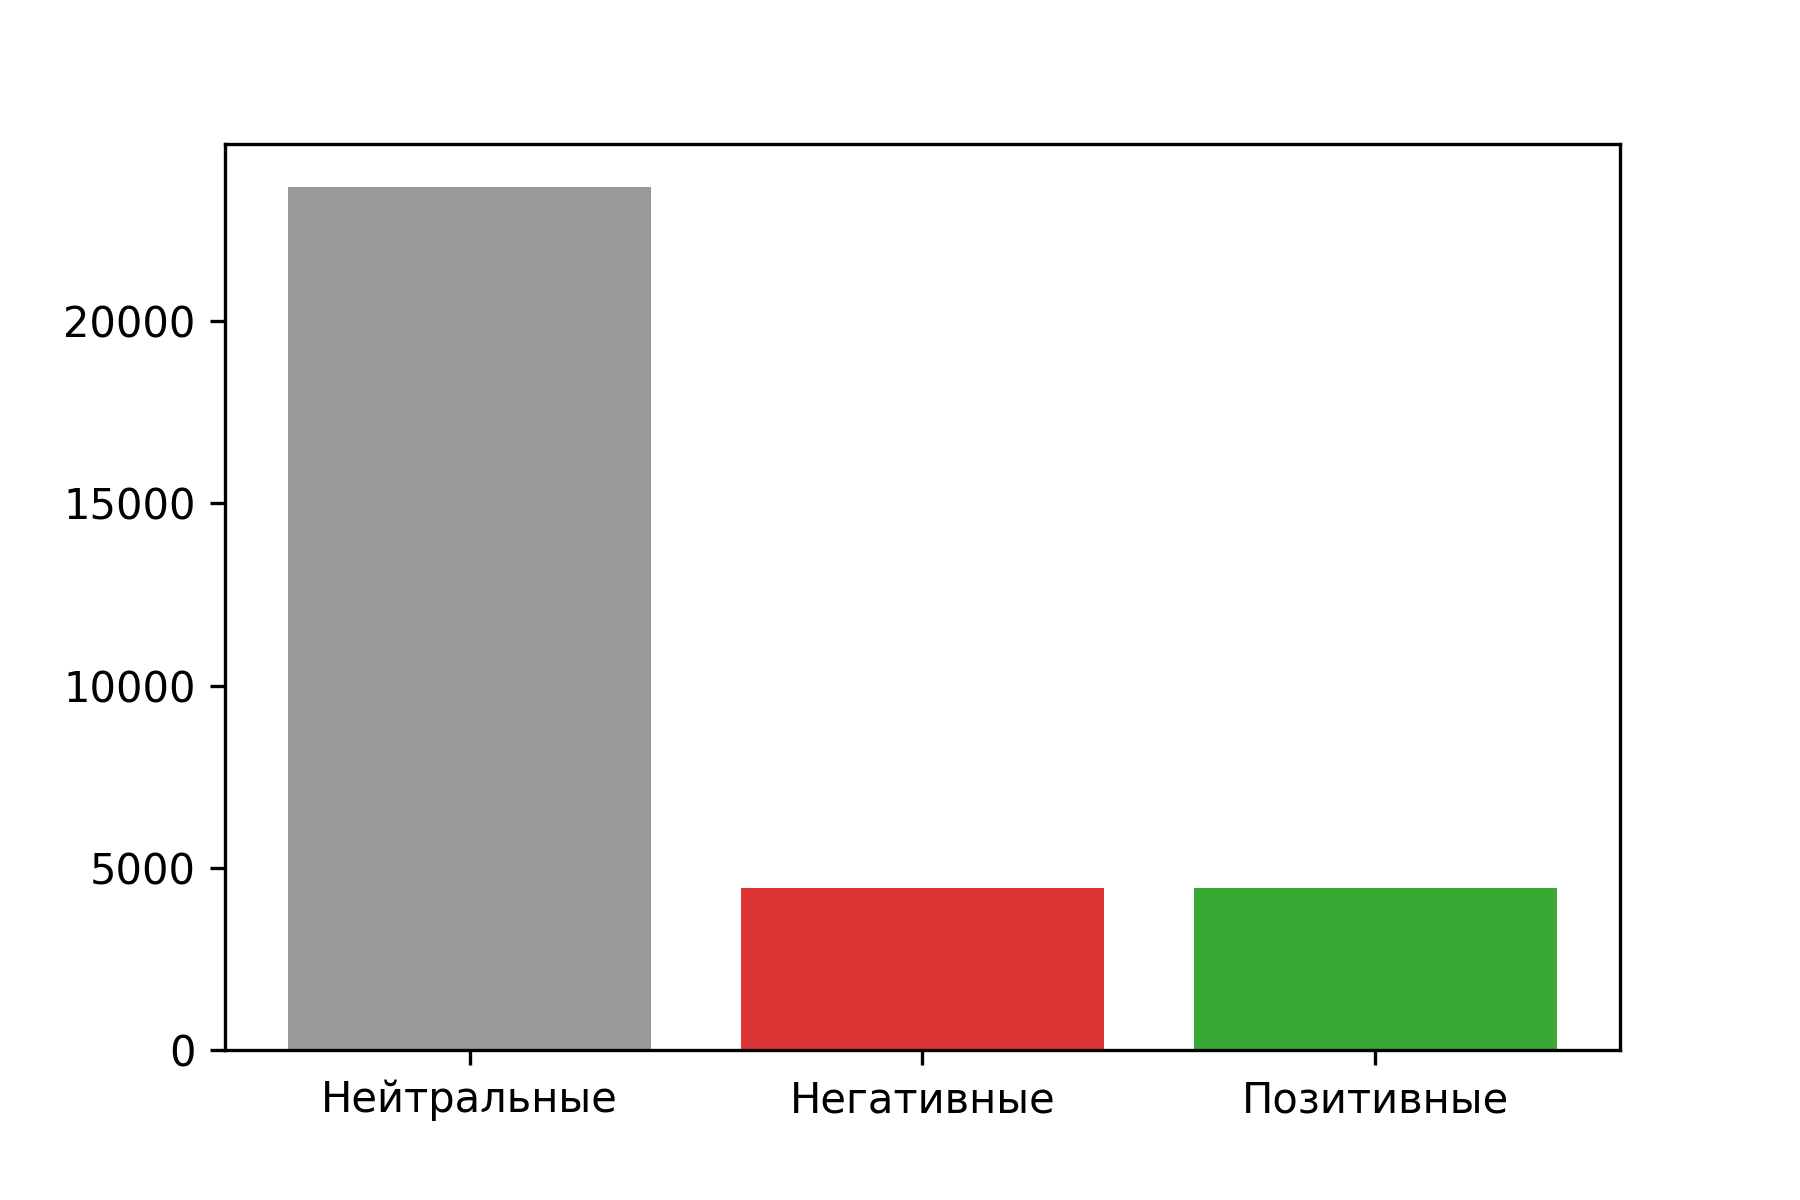
\includegraphics[scale=0.65]{imbalance.png}
	\caption{Распределение категорий в тренировочном наборе данных}
	\label{pic:imb}
\end{figure}

Особенности 3-4, обсуждаемые выше, будут активно приниматься во внимание при построении моделей.

\subsection{Представление данных}
Чтобы построить классификатор сообщений, нужно представить данные, понятным компьютеру образом. Более формально, нам необходимо определить пространство, из которого искомая модель $F(.)$ будет переводить сообщения в соответсвующие сентиментам классы. Имея численное представление каждого из предложений, можно применять математический аппарат к построению моделей. Принимая во внимание методы машинного обучения и статистики, такие представления могут задаваться самыми различными способами. В ходе исследования мы будем постепенно двигаться от простейших к более продвинутым, попутно делая выводы о преимуществах и недостатках каждого из подходов.

\subsubsection{OneHotEncoding}

OneHotEncoding $-$ один из множества способов определения множества значений, на котором будет работать искомая модель $F()$. Суть метода заключается в создании дамми-переменных в количестве, равном количеству слов в датасете. Таким образом, каждое сообщение можно закодировать вектором, состоящим из нулей и единиц. Единицы будут характеризовать наличие определенного слова, а нули $-$ отсутствие. Такой подход накладывает свои ограничения, среди которых:

\begin{enumerate}
	\item Необходимость хранения в оперативной памяти большого объема данных в процессе обучения алгоритма. В нашем случае, размер датасета, закодированного таким образом, имел бы размерность \[R^{\text{ Количество сообщений }\times\text{ Количество слов}} = R^{~31000\times 34733}\]
	\item Учитывая, что каждое слово кодируется единицей, получаем, что все слова имеют одинаковый вес. Однако, в русском языке некоторые слова встречаются гораздо чаще других, и их большее количество в тренировочных данных будет накладывать отпечаток на процесс оптимизации, о котором речь пойдет ниже. В качестве шага предобработки были предприняты меры по уменьшению количества лишних слов, но как можно видеть в таблице \ref{tab:table4}, среди наиболее употребительных слов все еще мелькают слова, не влияющие на сентимент сообщения.
\end{enumerate}

\subsubsection{Tf-Idf Encoding}
Tf-Idf $-$ решение проблемы равновзвешивания слов в процессе моделирования связи между сообщениями и их эмоциональным окрасом. Согласно этому подходу, каждому уникальному слову в тренировочном наборе данных соответствует определенный вес, исчисляемый по специальной формуле. Взвешивание слов должно решать главную проблему $-$ уменьшать значимость слов, которые не несут практического смысла. Как определить какое слово несет смысл, а какое нет? Создательница\footnote{Karen Spärck Jones. Synonymy and Semantic Classification — Edinburgh University Press., 1986. — Vol. 1. — (Edinburgh Information Technology series)} TF-IDF предложила следующую идею: если слово характерно не только для определенного сообщения, а для всего датасета в целом, то скорее всего, оно несет меньшую смысловую нагрузку, чем слово, которое встречается только в одном сообщении датасета. Чтобы отделить такие слова друг от друга, она придумала статистику, под названием TF-IDF, которая состоит из двух частей: TF (Term Frequency) и IDF (Inverse Document Frequency) и считается для каждого слова в отдельности. \[\text{TF-IDF}_{\text{i}} = TF_{\text{i}} \times IDF_{\text{i}} \quad \forall i  \text{ из словаря всех слов}\]
$TF_{i}$ часть отвечает за важность слова в пределах одного сообщения и рассчитывается по следующей формуле: \[ TF_{i} = \frac{n_{i}}{\sum\limits_{k=1}^{n}n_k} \]
где $n_i -$ количество повторений i-го слова в сообщение, а $n_k - $количество слов в одном сообщении.\\
$IDF_i$ отвечает за значимость слова в контексте всех сообщений в том смысле, о котором говорилось ранее: \[ IDF_i = \log \frac{|D|}{|{\{d_t \in D | i \in d_t\}}|}\] 
где $|D| - $количество всех сообщений, а $|\{d_t \in D | i \in d_t\}| - $количество сообщений, в которых встретилось i-ое слово. 
Получается, что для каждого слова мы считаем величину IDF, которая является единой для одинаковых слов и TF, которая разнится от предложения к предложению. Величина $TF-IDF$ тем больше, чем характернее слово для каждого из предложений. Среди проблемных мест такого численного представления слов можно выделить следующий:

\begin{enumerate}
	\item При кодировании теряется значение слов, определяемое порядком. К примеру, для TF-IDF, равно, как и для OneHotEncoding не существует разницы между предложениями <<Здесь сложно придумать что-то совершенно не бессмысленное>> и  <<Здесь не сложно придумать что-то совершенно бессмысленное>>.
\end{enumerate}

Разобравшись с возможностями представления слов в численном виде, мы смогли наглядно увидеть, как можно подготовить текстовые данные к тому, чтобы начать оценивать заветную модель \hyperref[eq:F]{(1)}. Настала пора перейти к самой интересной\footnote{Когда я проходил стажировку в одной из компаний занимающихся Data-Science, мой руководитель любил говорить, что выбор модели - награда за долгую и рутинную работу по предобработке данных.} части нашего исследования $-$ подбору модели. \\
Одно из негласных правил хорошего тона при любых исследованиях в сфере машинного обучения $-$ начинать с простейших моделей. Эта идея понятна: чем сложнее задача, чем сильнее желание попробовать что-то из ряда вон выходящее, но при рассмотрении сложных моделей, требующих более тонкой надстройки, исследователи, занимающиеся процессом оптимизации, зачастую не понимают, как хорошо работает их алгоритм. Можно видеть значения точности в районе $70\%$ успешно классифицируемых сообщений, однако совершенно непонятно, является ли это значение наилучшим, или, может быть, необходимо тратить кучу дополнительного времени на сбор дополнительных сообщений и их последующей разметки\footnote{Andrew Ng - известный исследователь в области машинного обучения и нейронных сетей. Его видеокурсы доступны на платформе coursera.org. На одной из своих лекций он рассказывал о компаниях, занимающихся применением ИИ в своих разработках, которые обращались к профессору за консультациями по исследованиям. Разработчики рассказывали о задаче, об алгоритмах которые они применяли, о результатах оптимизации и находились серьезные компании, которые не могли понять, почему их модели выходят на плато по точности и огромные временные и денежные затраты по добыче новых данных не исправляют проблем. Решением подобных ситуаций оказывалось сравнительная конкурентоспособность продвинутых алгоритмов с простейшими моделями. Руководители ИИ компаний, используя простейшие алгоритмы, получали бэнчмарки, нижние пороги по качеству моделей и понимали, что правильное направление - дооптимизация существующих алгоритмов.}. Начнем выбор модели с основных понятий. \\
\subsubsection{Основные понятия}
Подбор модели осуществляется в три этапа:
\begin{enumerate}
	\item Выбор оптимизируемой функции потерь. Эта специальное название функции, которая нужна, чтобы понимать, как хорошо наша модель отражает моделируемую зависимость. Функция потерь позволяет обучать алгоритмы.
	\item Выбор метрики качества. Эта метрика необходима, чтобы сравнивать между собой различные алгоритмы и интерпретировать потенциал обученной модели.
	\item Выбор непосредственно модели. Модель $-$ попытка формального построения связи между объектами исследования.
\end{enumerate}

\subsubsection{Функция потерь}
В парадигме подхода машинного обучения, подбор модели, отражающей исследуемую зависимость, осуществляется на основе постоянных наблюдений за влиянием изменений параметров модели на качество предсказания. Простыми словами, мы каким-то образом перебираем набор моделей и пытаемся понять, как хорошо та или иная модель отражают действительность. Учитывая особенности конкретно нашей модели (\ref{eq:F}), нам нужно учитывать, что сама модель переводит сообщения из некоторого пространства произвольной рамерности в 3-х мерное пространство эмоциональных состояний. В идеале, нам нужно предсказывать вероятности каждого из классов, причем предсказания каждого из классов образуют полную группу событий. Поэтому, избираемая функция потерь должна учитывать эту особенность. Кроме этого, вспомним об особенностях наших данных, заключающихся в несбалансированности классов. На такие запросы теория машинного обучения предлагает следующую функцию: \[ Loss(y, \hat{p}) = - \sum_{c=1}^{3} w_c y_c log(\hat{p}_c), \quad \text{где}\]
$w \in R^3 - $ вектор весов. \\
$y \in R^{3} - $ бинарный вектор метки класса определенного сообщения \\ $\hat{p} \in R^3 - $ вектор предсказания вероятностей сентимента для определенного сообщения \\\\
Напомню, что размерность вектора ответов для предсказываемого сообщения равна 3, потому что мы предсказываем вероятности каждого из 3-х классов сентимента. Вектор весов будет учитывать ошибку, совершаемую на несбалансированном классе сильнее, чем на доминирующем, чтобы мы не делали поспешных выводов о моделях с низкой функцией потерь, постоянно предсказывающих доминирующий класс. Итак, подытожим: процесс обучения будет сводиться к оптимизации функции потерь, путем перебора различных моделей. Чем меньше вероятность верного класса, тем выше значение функции потерь.

\subsubsection{Метрика качества}
Хорошая метрика качества должна оценивать предсказательную силу модели и давать ей интерпретацию. В случае многоклассовой классификации, предлагается следующий набор метрик:
\begin{enumerate}
	\item \emph{Accuracy} - показатель средней точности распознавания класса. Его основной недостаток заключается в отсутсвии чувствительности к несбалансированности. Высчитывается по следующей формуле: $\begin{aligned}[t]
	Accuracy(y, \hat{y}) = \frac{1}{n} \sum_{i=1}^{n}[y_i = \hat{y}_i]
	\end{aligned}$
	\item F-мера - статистика, не обладающая недостатком первой метрике. Высчитывается по формуле: \[ \text{F-мера} = 2\frac{precision \times recall}{precision + recall}}\]
\end{enumerate}
Остановимся поподробнее на F-мере. Представим, что после обучения на тренировочных данных мы хотим понять, как хорошо наша модель научилась видеть зависимости между словами и их сентиментами. Для этого мы делаем прогноз на отложенных данных и смотрим на результирующую матрицу ошибок, имеющую следующий вид: \\
\begin{figure}[h]
	\centering
	\begin{tabular}{l*{3}{c}r}
		Матрица ошибок         & Негативный & Нейтральный & Позитивный \\ 
		\hline
		Негативный            & 96 & 3 & 0   \\
		Нейтральный           & 6 & 650 & 1  \\
		Позитивный     & 6 & 2 & 115  \\
		
	\end{tabular}
\end{figure}

В матрице ошибок по столбцам описано количество реальных таргетов, а на их пересечении со строками $-$ количество предсказаний отнесенными классификатором к соответсвующему строке классу. Например, число 96 в матрице можно интерпетировать следующим образом: модель распознала 96 негативно окрашенных сообщений из 108. Построив такую матрицу, мы сможем определить две вещи: 1) точность алгоритма - доля сообщений, принадлежащих к верному классу; 2) полнота - доля предсказанных сообщений для верного класса в общей величине предсказанных классов. Первая вещь есть ничто иное, как Precision, а вторая - Recall. Контроль не только точности предсказания, но и отсутствия спутанности по предсказанию других классов объединяется в гармоническом среднем двух оценок - в F-мере. Такая форма объединения показателей гарантирует, что F-мера будет маленькой, если хотя бы один из показателей (Precision или Recall) будет маленький. Очень удобно.

 \subsubsection{Выбор моделей}
  \subsubsection*{Регрессия, как бэнчмарк}
Итак, обсудим, какими качествами должна обладать подходящая для нашей задачи модель:
\begin{enumerate}
	\item Переводить численное представление слов в вектор размерностью $R^3$, характеризующий вероятность каждого из классов. Поскольку сообщения должны быть классифицированы однозначно, сумма вероятностей каждого из классов складываются в единицу .
	\item Иметь набор параметров, изменяя которые, можно влиять на предсказания модели.
\end{enumerate}
Как и было заявлено в начале исследования - начинаем с простейших моделей. Рассмотрим основной регрессионный подход:
Пусть мы имеем матрицу данных размерностью $R^{31000 \times 34733}$. Напомню, что $31000 - $количество сообщений, а $34733 - $ количество уникальных слов в этих сообщениях. Для каждого из 31000 сообщений мы имеем вектор-строку вероятностей каждого из класса, например для нейтрального класса вектор-строка вероятностей имеет вид: \[ p = \begin{pmatrix} 1 & 0 & 0\end{pmatrix}\]
В действительности, если верен первый класс, то истинная вероятность того, что сообщение также принадлежит позитивному классу равна нолю. Это важный момент, потому что данная идея наводит на мысль о том, что какие бы предсказания в трехмерном пространстве не строила бы наша модель, значения соответсвующих вероятностей должны быть отнормированы таким образом, чтобы при суммировании вероятностей для каждого из наблюдений мы получали строгую единицу. Для этой цели в машинном обучении была придумана функция под названием <<Softmax>>

\begin{equation*}
Softmax(z_i) = \frac{e^{z_i}}{\sum\limits_{i=1}^{3}e^{z_i}}, \quad \text{ где}
\end{equation*}
$z \in R^3 - $ вектор предсказаний, построенный нашей моделью \\

Простейшая модель, генерирующая такой трехмерный вектор предсказаний является нейронная сеть, как на рисунке ниже. Предложения подаются в числовом представлении, одним из способов (OneHotEncoding или TF-IDF). Затем эти вектора умножаются на матрицы весов, таким образом, чтобы в результате умножения мы получили трехмерный вектор. Затем значения, выдаваемые этим трехмерным вектором нормируются softmax функцией. Весь этот цикл операций называется прямым проходом (forward pass) и математически представляется в следующем виде:
\begin{gather}
	\hat{p}_i = Softmax(X_iW + \beta) \\
	\hat{p}_i \in R^{(1, ~3)}, \quad X_i \in R^{(1, ~34733)} , \quad W \in R^{(34733, 3)}, \quad \beta\in R^{(1, 3)}\\
	Loss(y_i, \hat{p}_i) = -\sum_{c=1}^{3} y_{c_i} log(\hat{p}_{c_i})
\end{gather}

Отметим, что $\hat{p}_i$ - вектор вероятностей для $i$-го сообщения. После прохождения прямого прохода, мы считаем ошибку при помощи формулы (4) и обновляем параметры $W$ и $\beta$ таким образом, чтобы уменьшать значение функции ошибки на следующей итерации обучения. Способ обновления весов носит название градиентного спуска и предполагает обновление весов в соответствии с градиентом функции ошибки относительно каждого из параметров $W$ и $\beta$.

Процесс обновления весов формально:
\[ W_{t+1} = W_{t} - \alpha \frac{\partial Loss(W_t, \beta_t)}{\partial W_t} \]
\[ \beta_{t+1} = \beta_{t} - \alpha \frac{\partial Loss(W_t, \beta_t)}{\partial \beta_t} \]
 Такой подход обеспечивает постепенное уменьшение оптимизируемой функции потерь до определенного момента. Двигаясь в сторону антиградиента, рано или поздно мы дойдем до локального минимума функции ошибок. Параллельно с обучением, в конце каждой итерации происходит контроль значения функции ошибки на отложенной выборке, чтобы наблюдать за обощающей способностью алгоритма. 

 \subsubsection*{Дерево решений}
Еще одни алгоритм, который мы будем использовать помимо регрессионного подхода - использование дерева решений. Без лишних подробностей скажу только, что дерево работает по следующему принципу: на каждом итерационном шаге, алгоритм перебирает все слова из поданного на вход предложения и выбирает те, которые уменьшают кросс-энтропия путем полного перебора всех возможных слов. Кроме обычного дерева решений, существует случайный лес, состоящий, как можно было догадаться, из множества деревьев решений. У случайного леса есть одно важное преимущество - модель не запоминает данные, а вырабатывает обобщающую способность с ростом сложности оцениваемой структуры. \\ 
Сказав достаточно об используемых моделях перейдем к основным показателям, полученным в результате исследования:

\begin{figure}[h]
	\centering
	
	\begin{tabular}{ P{15mm} *{8}{P{12mm}} }
		\toprule
		& \multicolumn{4}{c}{One Hot Encoding} &  \multicolumn{4}{c}{TF-IDF} \\
		\cmidrule(lr){2-5}\cmidrule(lr){6-9}
		 & $Acc_{train}$ & $Acc_{test}$& $F1_{train}$ & $F1_{test}$ & $Acc_{train}$ & $Acc_{test}$& $F1_{train}$ & $F1_{test}$  \\
		\midrule
		Нейросеть  & 0.853 &  0.724 & 0.771 &0.559  &  0.804 &  0.732 & 0.690  &  0.567 \\
		Лес  & 0.984 & 0.736  &0.977 &0.530  & 0.989  & 0.744  & 0.983   & 0.507  \\
		Дерево  & 0.785 & 0.554  &0.741 &0.458  &  0.890 & 0.614  & 0.856  & 0.472  \\
		\bottomrule
	\end{tabular}
\caption{Результаты тестирования различных моделей}
\end{figure}

Как можно видеть из результатов, наилучшие показатели по нашей основной метрике качества F-мере демонстрирует нейросеть. Можно было бы выбрать её в качестве основной модели и использовать, но здесь есть один очень важный момент. Что общего между всеми этими подходами? И нейронная сеть, и дерево решений, и случайный лес,- все модели используют в качестве данных статистики, полученные из тренировочного датасета. Простым языком, если мы будем использовать слова, которые отличаются от слов, присутствовавших в исходном датасете (не формой слова, а написанием), то будем терять информацию с этих слов, просто потому что ни One Hot Encoding пространство, ни TF-IDF не способны дать существенную информацию о новых словах. Как же нам быть? На помощь приходят современные нейросетевые алгоритмы. 
В 2013 году миру была представлена модель\footnote{Distributed Representations of Words and Phrases and their Compositionality, https://papers.nips.cc/paper/5021-distributed-representations-of-words-and-phrases-and-their-compositionality.pdf}, изменившая представление вещей на долгие годы вперед. Группа исследователей из компании Google выяснили, что если, имея все знания мира, попытаться отдать их нейросети в текстовой форме, то последняя сможет построить векторное пространство всех слов в соответствии с их семантическим взаимотношением. Конечно, понятия <<отдать знания нейросети>> подразумевают постановку специальной задачи и куда более специфичные технические тонкости, но основной смысл состоит в том, что в 2013 году мир получил возможность черпать знания о словах извне. Есть прекрасные современные ресурсы, демонстрирующие то, что я имею в виду\footnote{https://rusvectores.org/ru/}. Как это открытие повлияет на наше решение? Очень просто: отныне и впредь мы будем переводить слова в векторы не при помощи One Hot Encoding или TF-IDF подхода, а при помощи предобученных векторов. Мы будем использовать эти предобученные вектора с той целью, чтобы при появления синонимичного слова, отсутствовавшего в нашем тренировочном датасете, модель не выкидывала что-то нелогичное, а относилась бы к этому слову, как к синониму какого-нибудь другого слова из тренировочного набора данных. Надо сказать, что само по себе добавление знания о внешнем мире не увеличило точность модели на отложенной выборке, но при подробном приближении, мы заметили, что необычные слова классифицируются правильнее с использованием обученного векторного пространства, чем при помощи OHE или TF-IDF. Последние имели тенденцию к <<занейтраливанию>> сообщения.

\section{Тестирование полученной информации}
\label{sec:portfolio}
Создав языковую модель перевода сообщений в их сентименты, мы вольны что-угодно творить с полученными рядами данных (см. таблицу \ref{tab:table5} в приложении). Для начала выдвенем основные гипотезы, относительно возможных связей полученных данных со стоимостью котировок. Логично предположить, что если люди говорят много хорошего про бумагу, то скорее всего она будет расти. Аналогичное верно и для обратного: если сказано много плохого, то скорее всего стоимость бумаги начнет падать. Кроме того, вероятно, степень влияния сентиментов сильнее для компаний с маленькой капитализацией, по сравнению с компаниями большей капитализации. Данные гипотезы мы будем тестировать при помощи симуляции портфелей.\footnote{Идея тестировать гипотезы таким образом принадлежит Александру Томтосову, моему коллеге по научной лабаратории. Моя роль в симуляции заключалась в автоматизации процессов.}
В ходе этого исследования проводилась симуляция портфелей ценных бумаг, отобранных по специальным метрикам, которые, в свою очередь, базировались на показателях сентиментов. Симуляция портфеля проходила в следующие этапы:

\begin{enumerate}
	\item Отбирались 60 компаний. Отбор происходил по размеру компаний: по 20 штук для малой, средней и высокой капитализации.
	\item На основе сентиментов строились фильтры, согласно которым, каждый месяц определялись лидеры в каждой из групп капитализации.
	\item Компании-лидеры покупались и держались ровно месяц. За этот месяц фиксировался результат доходности портфеля, после чего следовала ребалансировка (повторение шага 2).
\end{enumerate}

Какие же фильтры использовались для ребалансировки портфелей?
\subsubsection*{Спецификация фильтров}
\subsubsection{Количество положительных сообщений} Основная гипотеза состоит в том, чтобы покупать бумаги с наибольшим количеством положительных отзывов. Как уже отмечалось ранее, чем больше положительных отзывов имеет бумага, тем возможно больше внимания она привлекает со стороны. Учитывая специфику разметки данных, можно сказать, что положительные комментарии о бумаге включают также фразы по типу <<я закупился>> или <<тарю>>. Можно сказать, что количество положительных сообщений являются в какой-то степени являются прокси для измерения спроса на бумагу. 

\subsubsection{Дивергенция мнений}
Идея состоит в том, что независимо от того, как соотносятся позитивные и негативные настроения инвесторов, если они разрозненны, то состояние рынка неопределено. Если инвесторы достигают консенсуса в выборе направления движения рынка, то либо они 1) одновременно сходятся во мнении о благоприятной для инвестирования обстановке, 2) либо они одновременно лгут о негативной обстановке, чтобы повыгоднее войти на рынок. Формула для расчет дивиргенции представлена ниже:

\begin{equation*}
	Divergence = \sqrt{\frac{(n_{pos} - n_{neg})^2}{(n_{pos} + n_{neg})^2}}
\end{equation*}\\
$n_{pos} -$  количество позитивных сообщений \\
$n_{neg} -$  количество негативных сообщений

\subsubsection{Количество отрицательных сообщений}

Гипотеза состоит в том, что, если рынок слишком сильно раскритикован, если каждый говорит о том, что все плохо, то скорее всего частный инвестор воздержится от покупки бумаг. Заметим, что конечное предположение качественно отличается от предыдущего пункта.

\subsubsection{Доля сообщений по компании в величине всех сообщений}

Логика здесь следующая: возможно, что некоторые инвесторы перед покупкой определяют степень популярности бумаги и берут только те, которые обсуждаются больше всего.


\subsubsection{Среднеквадратичное отклонение доходности внутри месяца}

Данный фактор берется скорее в качестве бенчмарка в расчете на то, чтобы сравнить показатели доходности портфеля от ребалансировки при помощи отобранных сентиментов. Считается, как стандартное отклонение доходности бумаги.

\subsubsection{Суммарный объем торгов по акции}

Аналогично вышестоящему фактору, берем этот фактор как бенчмарк по отношению к нашему подходу. В исследовании интересно получить сравнительные результаты, нежели чем просто результаты.

\subsubsection{Изменение цены закрытия к предыдущему периоду}
Известная среднесрочная стратегия. Посмотрим, дадут ли сентименты возможность получить доходность большую, чем эта стратегия. Моментум считается по формуле:

\begin{equation*}
	m_{t+1} = \frac{P_{t+1}}{P_{t}} - 1
\end{equation*}

Каждый из вышеперечисленных факторов использовался в определении состава портфелей следующим образом:

\begin{enumerate}
	\item Для каждой бумаги, для каждой из групп капитализации, для каждого временного промежутка считался каждый из вышеперечисленных факторов. 
	\item В момент принятия решения о выборе бумаг для портфеля, каждая из компаний, внутри своей группы капитализации, ранжировалась по убыванию факторов.
	\item Затем составлялся портфель по топ-$50\%$ компаниям для каждой из групп факторов в рамках разных капитализаций.
	\item Эти компании покупались в равной пропорции, формируя общую доходность портфеля.
	\item Вышеописанная процедура повторялась каждый месяц. Каждая из отобранных бумаг имела равный вес в портфеле.
\end{enumerate}
В ходе таких симуляций были получены следующие результаты:

\begin{figure}[h]
	\centering
	
	\begin{tabular}{P{19mm} *{8}{P{14mm}} }
		\toprule
		& \multicolumn{4}{c}{Mean Excess Return} &  \multicolumn{4}{c}{Mean Monthly Return} \\
		\cmidrule(lr){2-5}\cmidrule(lr){6-9}
		& $All$ & $Low$& $Mid$ & $Lrg$ & $All$ & $Low$& $Mid$ & $Lrg$ \\
		\midrule
		Позитив  & 0.9 (2.05)** &  1.74 (1.04) & 0.56 (1.19)  &0.44 (1.09)   &  2.5 (3.32)*** &  4.2 (1.98)* & 1.6 (2.09)**  &  1.75 (3.36)*** \\

		Негатив  & 0.83 (1.9)* & 0.55 (0.44)   &1.68 (2.86)*** &-0.13 (-0.32)   & 2.43 (3.33)***  & 3.02 (1.95)*  & 2.72 (3.36)***   & 1.18 (2.21)**  \\ 
		Сумма  & 0.68 (1.67)* & 0.29 (0.24)   &0.47 (0.94)  &0.13 (0.39)   &  2.28 (3.51)*** & 2.75 (1.8)*  & 1.51 (2.09)**  & 1.44 (2.56)**  \\ 
		Дивергенция  & 0.11 (0.33)  & 0.57 (0.41)   &0.24 (0.52)  &-0.27 (-0.75)   &  1.72 (2.35)** & 3.03 (1.64)   & 1.28 (1.6)   & 1.04 (1.49)   \\ \cmidrule{1-9}
		Momentum  & 1.36 (2.56)** & 0.92 (0.7)   &0.93 (1.62)  &0.82 (1.7)*  &  2.96 (3.3)*** & 3.38 (2.05)**  & 1.97 (2.09)**  & 2.12 (3.26)***  \\ 
		Relative  & 0.5 (1.25)  & 0.32 (0.26)   &0.46 (0.93)  &0.08 (0.23)   &  2.11 (3.29)*** & 2.78 (1.79)*  & 1.5 (2.09)**  & 1.39 (2.45)**  \\ 
		Volatility  & -0.04 (-0.13)  & -1.05 (-0.92)   &-0.09 (-0.17)  &-0.05 (-0.11)   &  1.56 (2.31)** & 1.41 (0.99)   & 1.41 (0.99)   & 1.26 (1.81)*  \\
		Volume  & 0.43 (0.99)  & 0.19 (0.14)   &0.87 (1.49)  &-0.26 (-0.66)   &  2.03 (2.75)*** & 2.66 (1.62)   & 1.91 (2.08)**  & 1.05 (1.65)   \\
		\bottomrule
	\end{tabular}
\caption{Результаты симуляций портфеля}
\label{tab:winners}
\end{figure}

Данную таблицу следует понимать следующим образом. Первая группа результатов Mean Excess Return показывает насколько доходность симулированной стратегии больше доходность равновзвешенного держания 20 компаний в своем портфеле. Простым языком, это значит следующее: предположим, на рынке есть два трейдера, первый из них торгует по стратегии, которую мы описали выше, а второй просто закупает каждый месяц по 20 бумаг и в конце каждого месяца их продает. Вот если посмотреть, насколько статистически первый заработает больше второго, то мы получим результаты, описанные в этой половине таблицы. Из данных видно, что трейдер, каждый месяц покупавший по 10 бумаг средней капитализации, опираясь на количество самых негативно-обсуждаемых бумаг (пересечение строки Негатив и столбца Mid в секции Mean Excess Return) зарабатывал ежемесячно на 1.68\%  больше трейдера второго типа из нашего примера. Для того, чтобы понять, а какую же доходность приносил портфель первого трейдера, обратимся ко второй секции таблицы. На пересечении строки Негатив и столбца Mid мы видим число 2.72\%, характеризующее среднемесячную доходность портфеля. Среднемесячная доходность в 2.72\% кажется невероятно большой. Посмотрим на изменения в стоимости портфеля:

\begin{figure}[h]
	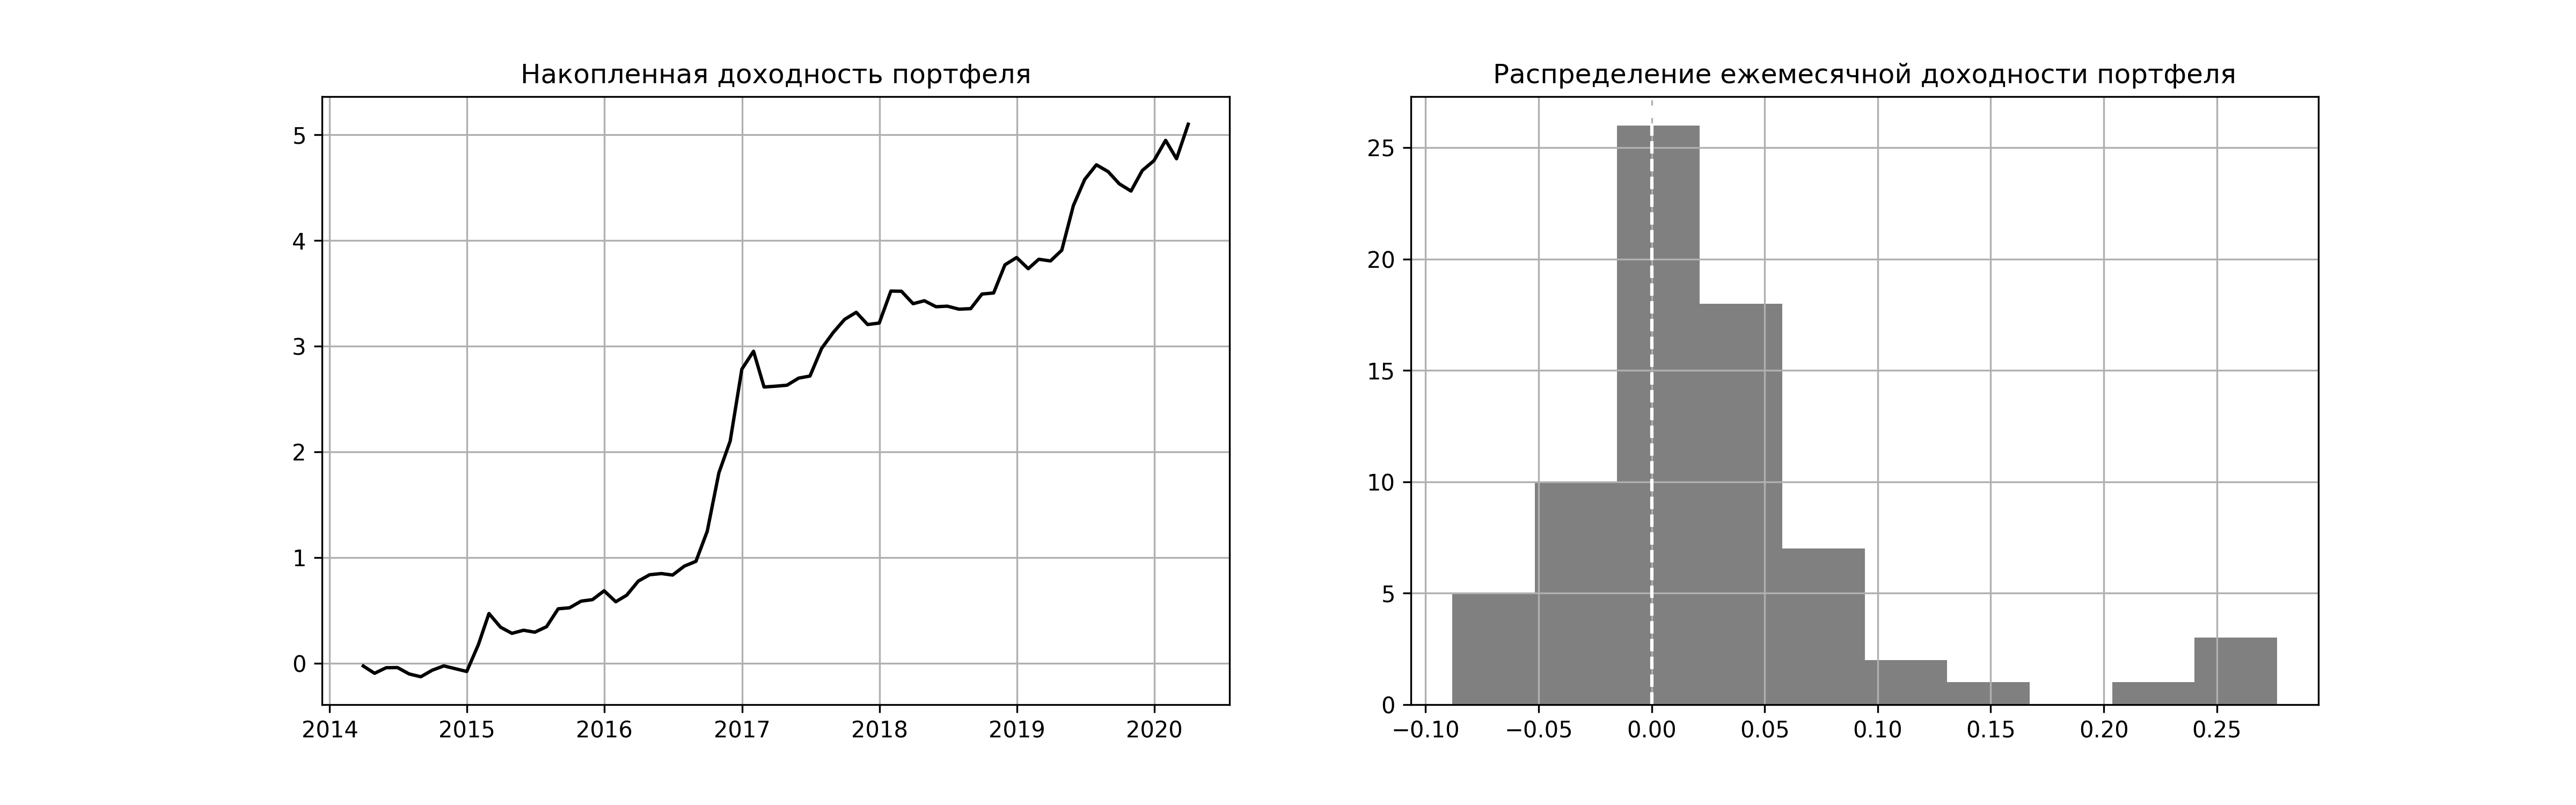
\includegraphics[scale=0.4]{portfel.png}
	\caption{Изменение стоимости портфеля}
\end{figure}

Обратим внимание на колосальный рост стоимости портфеля в промежутки с середины 2016 по 2017 год и его крайне низкую волатильность. Интересно посмотреть, что за бумаги так сильно повлияли на стоимость портфеля и чем был опеспечен прирост. Для этого я рассмотрел построенный портфель в период с 2016-го по начало 2017-го года и нарисовал топ-10 самых <<Hated>> компаний, которые люди с форума mfd, топили и ненавидели больше всего: 

\begin{figure}[h]
	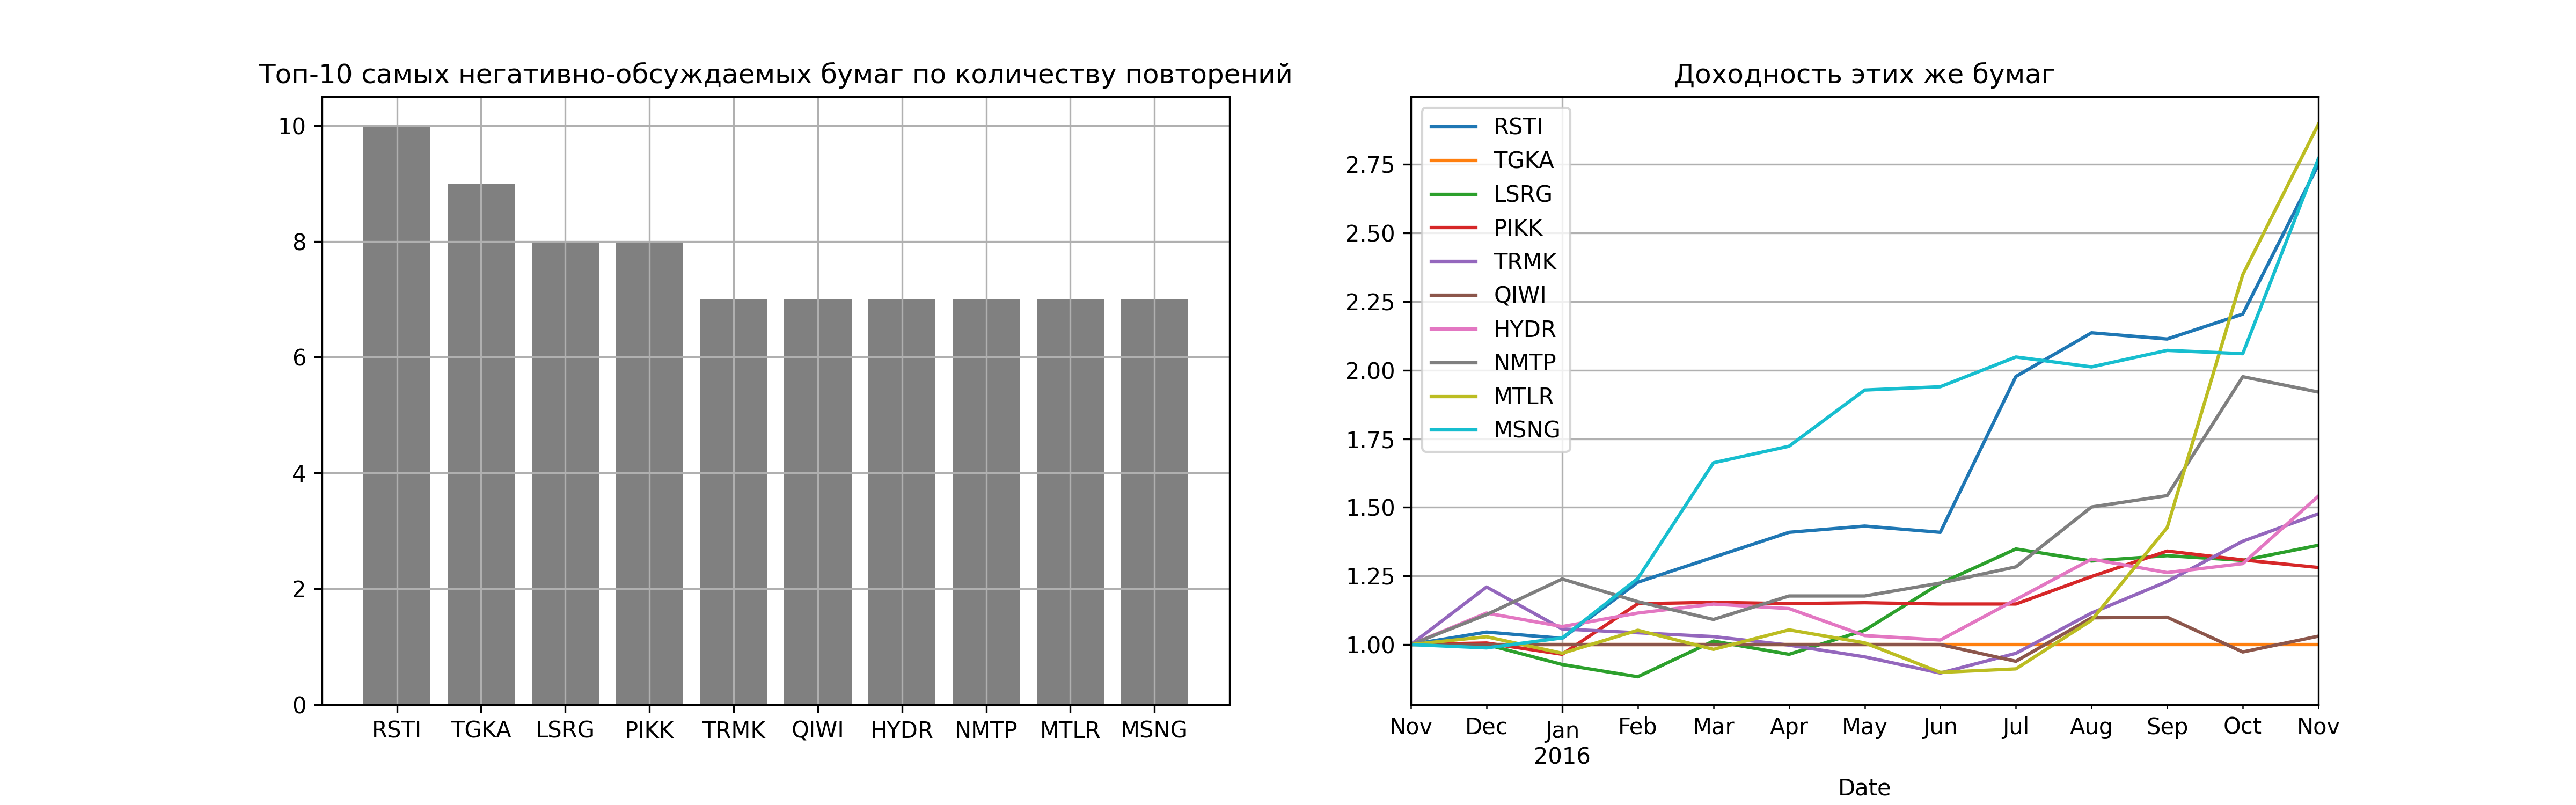
\includegraphics[scale=0.4]{rofl.png}
	\caption{Изменение стоимости самых негативно-обсуждаемых бумаг}
	\label{fig:rofl}
\end{figure}

На столбчатой диаграмме (Рис. \ref{fig:rofl}) можно увидеть топ-10 самых ненавистных компаний. По оси-$oY$ расписано количество раз, когда компания избиралась в портфель по показателю негатива. А на графике справа $-$ изменение в стоимости соответствующих бумаг. Какие выводы из этого можно сделать? Эти графики явно показывают ту долю скептицизма, с которой нужно относиться к сказанному негативу на финансовых форумах.  \\

Проинтерпертируем другие полученные результаты. Положительная избыточная доходность также наблюдается для стратегии моментум, для компаний из группы большой капитализации. Исходя из таблицы, следование данной стратегии приносило бы ежемесячно в среднем 2.12\%, что больше бэнчмарка в среднем на 0.82\%. \\
Кроме вышесказанного, можно заметить, что значимость в избыточной доходности присутствует в объединенной группе компаний (столбец All в таблице выше). Эта группа подразумевает, что теперь в схеме отбора участвовали компании с разными капитализациями все вместе. Значимость позитива, негатива и суммы сообщений для всех компаний означает следующее: построение портфеля из топ-$50\%$ бумаг по российскому рынку, при использовании этих факторов позволяет заработать на $0.68\% - 0.9\%$ ежемесячно больше рынка. Общая месячная доходность таких портфелей составила бы $2.28\% - 2.5\%$ соответственно. \\

Что бы изменилось, если бы теперь мы строили портфели, покупая не лидеров по указанным фильтрам, а аутсайдеров? Основные гипотезы тогда бы имели следующую форму:

\begin{enumerate}
	\item <<Греби лихо пока тихо>>. Есть смысл покупать бумаги, про которые говорят меньше всего негатива. Маленький негатив $\to$ покупаем.
	\item Бурное обсуждение ни к чему не приводит. Есть смысл покупать только те бумаги, о которых мало говорят. Меньше всего сообщений $\to$ покупаем
	\item <<Слишком хорошо $- $ тоже плохо>>. Меньше всего положительных отзывов $\to$ покупаем.
	\item Большой разброс мнений, как сигнал к покупке. Маленькая дивергенция  $\to$ покупаем.
\end{enumerate}

Тестирования данных гипотез привело к получению следующих результатов:

\begin{figure}[h]
	\centering
	\begin{tabular}{P{19mm} *{8}{P{14mm}} }
		\toprule
		& \multicolumn{4}{c}{Mean Excess Return} &  \multicolumn{4}{c}{Mean Monthly Return} \\
		\cmidrule(lr){2-5}\cmidrule(lr){6-9}
		& $All$ & $Low$& $Mid$ & $Lrg$ & $All$ & $Low$& $Mid$ & $Lrg$ \\
		\midrule
		Позитив  & -0.45 (-1.36)  &  -1.71 (-2.04)** & -0.33 (-0.7)   &-0.05 (-0.1)    &  1.15 (1.74)* & 0.75 (0.78)  & 1.26 (1.55)   &  0.7 (1.12)  \\
		
		Негатив  & -0.71 (-2.05)** & -1.79 (-2.18)**   &-0.49 (-0.99)  &-0.09 (-0.22)    & 0.89 (1.3)   & 0.67 (0.81)  & 0.55 (0.83)    & 1.22 (1.64)  \\ 
		Сумма  & -0.75 (-2.43)** & -1.82 (-2.17)**   &-0.82 (-1.89)* &0.06 (0.14)    &  0.86 (1.37)  & 0.64 (0.72)   & 0.22 (0.37)   &1.37 (1.71)*  \\ 
		Дивергенция  & 0.22 (0.66)   & 0.35 (0.33)    &-0.48 (-1.11)   &0.4 (1.05)    &  1.82 (2.89)*** & 2.81 (2.27)**  & 0.56 (0.75)    & 1.71 (2.6)**   \\ \cmidrule{1-9}
		Momentum  &-0.94 (-2.47)** & -1.29 (-1.23)    &-0.57 (-1.0)   &0.35 (0.81)   & 0.66 (0.95)  & 1.17 (0.88)   & 0.47 (0.54)   & 1.66 (2.15)**  \\ 
		Relative  & -0.7 (-2.28)**  & -1.6 (-1.91)*  &-0.83 (-1.93)*  &0.06 (0.14)    &  0.91 (1.45)  & 0.87 (1.0)   & 0.21 (0.35)   & 1.37 (1.71)*  \\ 
		Volatility  & -0.08 (-0.22)   & -1.98 (-2.55)**  &0.24 (0.54)  &-0.07 (-0.18)    &  1.53 (2.19)** & 0.48 (0.54)   & 1.28 (1.62)    & 1.24 (1.68)*  \\
		Volume  & -0.04 (-0.08)   & 1.67 (0.95)    &-0.54 (-1.2)   &-0.61 (-1.49)   &  1.57 (1.81)* & 4.13 (1.77)*   & 0.5 (0.79)  & 0.7 (0.92)    \\
		\bottomrule
	\end{tabular}
	\label{tab:losers}
	\caption{Результаты симуляций портфеля при покупке аутсайдеров }
\end{figure}

Из таблицы видно, что покупка аутсайдеров ни к чему хорошему не приводит $-$ избыточная доходность для значимых показателей отрицательна. Увы, ни одна из сформулированных гипотез не оправдалась. \\

\section{Выводы}
\label{sec:conclusion}
В ходе данного исследования при помощи методов машинного обучения и статистики были обнаружены взаимосвязи между сообщениями с финансовых форумов и изменениями в стоимости акций. Анализ влияния негатива на поведение инвесторов позволяет сделать вывод о том, что сбор информации по пессимистичности людей может объяснять часть изменений в доходности бумаги. Моделирование русского языка позволило получить на практике инструмент к созданию индекса <<негативности>>. Формирование портфеля на основе негативных отзывов позволило получить значимую ежемесячную доходность в размере 2.72\%.



\newpage
\section{Приложение}


\label{chap:additional}


\begin{table}[h]
	\caption{Частотность первых и последних 20 слов после обработки}
	\label{tab:table4}
	\centering
	\begin{tabular}{llll}
		\toprule
		%Заголовки
		Слово & Частотность слова &Слово & Частотность слова\\
		\midrule
		не & 13517 & marketbeat & 1\\ 
		а & 6964 & bmo & 1\\ 
		эт & 4206 & canad & 1\\ 
		год & 2402 & raymond & 1\\ 
		шорт & 1807 & james & 1\\ 
		быт & 1654 & canaccord & 1\\ 
		сегодн & 1626 & genuit & 1\\ 
		ден & 1626 & cibc & 1\\ 
		так & 1517 & mull & 1\\ 
		нефт & 1507 & торонт & 1\\ 
		рост & 1499 & акр & 1\\ 
		цен & 1442 & мобилизова & 1\\ 
		акц & 1334 & скептичн & 1\\ 
		дума & 1265 & финанасов & 1\\ 
		пок & 1241 & недопустим & 1\\ 
		див & 1219 & гсп & 1\\ 
		рынок & 1184 & xi & 1\\ 
		дава & 1163 & неаффилирова & 1\\ 
		сво & 1159 & неаффилирован & 1\\ 
		компан & 1059 & несоответств & 1\\
		\bottomrule
	\end{tabular}
	\label{tab:table3}
\end{table}

\begin{figure}[!h]
	\centering
	\caption{Простейшая нейронная сеть}
	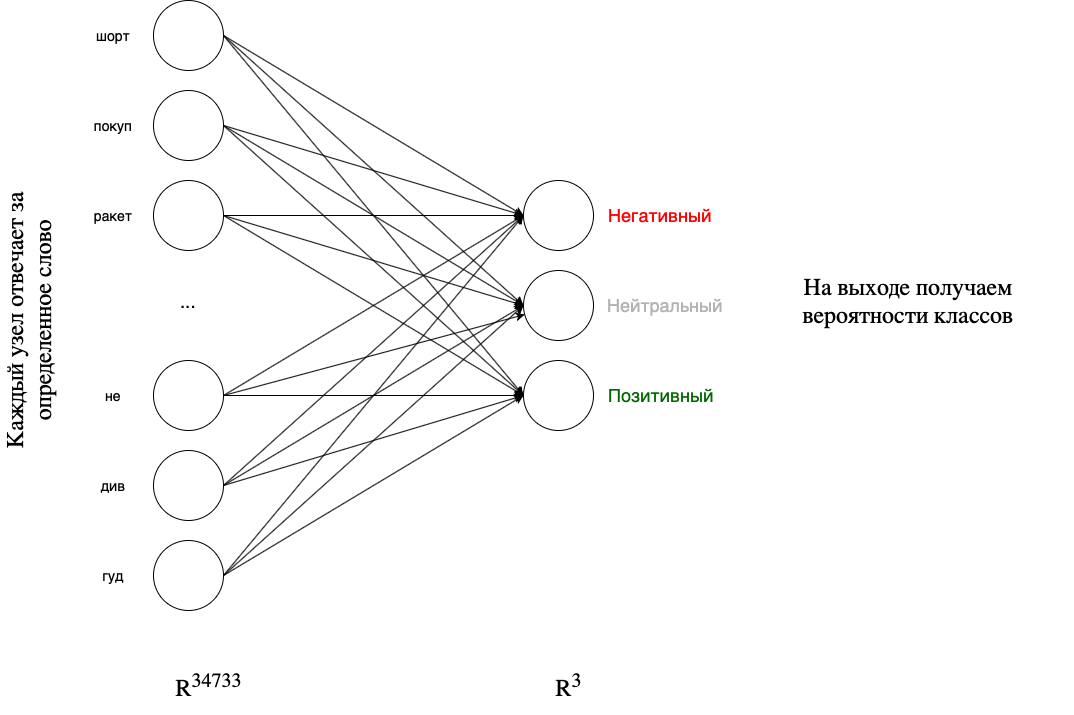
\includegraphics[scale=0.3]{nn.png}
\end{figure}


\begin{table}[!h]
	\caption{Данные после распознавания сентимента}
	\label{tab:table5}
	\centering
	\begin{tabular}{llll}
		\toprule
		%Заголовки
		Дата & Негативных & Нейтральных & Позитивных \\
		\midrule
		2013-02-11 & 44 & 67 & 18  \\ 
		2013-02-12 & 154 & 263 & 89  \\ 
		2013-02-13 & 110 & 215 & 59  \\ 
		2013-02-14 & 112 & 147 & 47  \\ 
		2013-02-15 & 35 & 74 & 20  \\ 
		2013-02-16 & 18 & 34 & 11  \\ 
		2013-02-17 & 8 & 21 & 6  \\ 
		2013-02-18 & 44 & 121 & 30  \\ 
		2013-02-19 & 43 & 80 & 25  \\ 
		2013-02-20 & 17 & 50 & 12  \\ 
		2013-02-21 & 18 & 14 & 12  \\ 
		2013-02-22 & 57 & 55 & 13  \\ 
		2013-02-23 & 3 & 10 & 0  \\ 
		2013-02-24 & 0 & 2 & 0  \\ 
		2013-02-25 & 29 & 77 & 22  \\ 
		2013-02-26 & 27 & 73 & 12  \\ 
		2013-02-27 & 23 & 85 & 20  \\ 
		2013-02-28 & 24 & 66 & 6  \\ 
		2013-03-01 & 15 & 29 & 11  \\ 
		2013-03-02 & 7 & 14 & 6  \\ 
		\bottomrule
	\end{tabular}
\end{table}


\begin{table}[h]
	\centering
	\caption{Группы компаний для анализа}
	\label{tab:table6}
	\begin{tabular}{lcllcllcll}
		
		\multicolumn{2}{c}{Маленькая капитализация} & \multicolumn{2}{c}{Средняя капитализация} &  \multicolumn{2}{c}{Крупная капитализация} \\ 
		\toprule
		Компания& Объем &Компания& Объем&Компания& Объем     \\ \midrule
		НКНХ& 176.5 & Уралкалий&  248.0 & Газпром&  4766   \\
		 Черкизово & 75.7  & Распадская&32.6 & Сбербанк& 4786    \\ 
		  Ленэнерго & 67.6 &ЛСР&   63.5 & Лукойл& 3778 \\
		  Иркут & 42.2&Мечел& 41.4 & Норникель& 3156   \\
		   Ятэк & 33.0&Фосагро&  364.7 &Татнефть& 1297  \\
		  Аптеки 36 и 6& 32.0  &Ростелеком&  234.5 &Сургутнефтегаз& 1686  \\
		   Селигдар & 21.8 &Россети&  320.5 &Роснефть&4134  \\
		 КТК& 15.7 &Русгидро&  307.5 &ВТБ& 1001  \\
		 Сар. НПЗ  & 14.5&Система&  165.8 &Алроса& 490.1  \\
		  Русолово & 11.8 &ТМК& 61.4 & Мосбиржа&268.3   \\
		   Соллерс   & 8.81  &Юнипро& 175.2 & Яндекс&945.1   \\
		 ГАЗ   & 7.29 &Акрон& 241.3 &Аэрофлот&95.5   \\
		 Ашинский& 2.01 &ПИК& 255.6 &ФСК ЕЭС&234.1   \\
		   ЧЗПСН & 1.38 &Лента& 79.3 &ММК&474.5   \\
		    Дагсбыт & 0.51 &Мосэнерго&  86.2 &МТС&645.3  \\
		  Арсагера  & 0.40&ТГК-1&   50.3 &Новатэк&3253 \\
		  GTL& 0.24  &Русал&   409.1 &НЛМК& 829.5 \\
		     Тантал & 0.24  &Транснефть&   1196 &Северсталь&790.3 \\
		 Роллман& 0.12 &Газпромнефть&  1636 &Магнит&390.4  \\		 		 
		   Сиб. Гостинец& 0.04  &НМТП&   182.0 &Полюс&1420 \\		 
		 \bottomrule
		
	\end{tabular}
\end{table}



\newpage
\bibliographystyle{unsrt}  
%\bibliography{references}  %%% Remove comment to use the external .bib file (using bibtex).
%%% and comment out the ``thebibliography'' section.


%%% Comment out this section when you \bibliography{references} is enabled.
\begin{thebibliography}{1}

\bibitem{2014oli}
Nuno Oliveira, Paulo Cortez, Nelson Areal.
\newblock The impact of microblogging data for stock market prediction: Using
Twitter to predict returns, volatility, trading volume and survey
sentiment indices
\newblock In {\em Expert Systems With Applications 73 (2017)}, p. 125-144.

\bibitem{2017ren}
Thomas Renault.
\newblock Intraday online investor sentiment and return patterns in the U.S.
stock market,
\newblock In {\em Journal of Banking and Finance, 2017 84th} (2017), p. 25-40. 

\bibitem{arxiv-sent}
\newblock Paolo Cremonesi, Chiara Francalanci, Alessandro Poli, Roberto Pagano, Luca Mazzoni, Alberto Maggioni, Mehdi Elahi.
\newblock \emph{<<Social Network based Short-Term Stock Trading System>>} (2018)
\newblock arXiv:1801.05295 [cs.SI]

\bibitem{2019chi}
Thi-Thu Nguyen and Seokhoon Yoon.
\newblock <<A Novel Approach to Short-Term Stock Price
Movement Prediction using Transfer Learning>>,
\newblock In {\em Journal Applied Sciences, 2019 9th}, p. 3-16.

\bibitem{123}
Qurat Tul Ain, Mubashir Ali.
\newblock 	<<Sentiment Analysis Using Deep Learning Techniques: A Review>>
\newblock (IJACSA) International Journal of Advanced Computer Science and Applications, Vol. 8, No. 6, (2017)

\bibitem{aplsci_port}

\newblock Van-Dai Ta, CHUAN-MING Liu and Direselign Addis Tadesse. 
\newblock <<Portfolio Optimization-Based Stock Prediction Using Long-Short Term Memory Network in Quantitative Trading>> (2020)
\newblock Applied Sciences (Internet Journal)


\bibitem{arxiv_twitter}

\newblock Ellie Birbeck and Dave Cliff.
\newblock <<Using Stock Prices as Ground Truth in Sentiment Analysis to Generate Profitable Trading Signals>> (2018)
\newblock arXiv:1811.02886 [cs.CE]

\bibitem{1234}
\newblock Lei Zhang, Shuai Wang, Bing Liu (2018)
\newblock <<Deep Learning for Sentiment Analysis: A Survey>> (2018)
\newblock arXiv:1801.07883 [cs.SI]

\bibitem{12345}
\newblock Alpna Patel and Arvind Kumar Tiwari.
\newblock <<Sentiment Analysis by using Recurrent Neural Network>>
\newblock $ 2^{nd} $ International Conference On Advanced Computing And Software Engineering (Icacse-2019) (2019), p. 108-111

\bibitem{123456}
\newblock Panchenko A. I.
\newblock <<Sentiment Index of the Russian Speaking Facebook>> (2018)
\newblock arXiv:1808.07851 [cs.SI]


\bibitem{12345678}
\newblock Chetviorkin, Ilia, and Natalia Loukachevitch. <<Evaluating Sentiment Analysis
Systems in Russian>>, ACL 2013 (2013), p. 12-17

\bibitem{821399}
\newblock Mihalcea, Rada, and Hugo Liu. <<A Corpus-based Approach to Finding Happiness>>.
AAAI Spring Symposium: Computational Approaches to Analyzing Weblogs (2006).

\bibitem{2918}
\newblock Godbole, Namrata, Manja Srinivasaiah, and Steven Skiena. <<Large-Scale Senti- ment Analysis for News and Blogs>>. ICWSM 7, (2007)

\bibitem{wdawdo}
\newblock Blinov P., Klekovkina M., Kotelnikov E., Pestov O. <<Research of lexical approach and machine learning methods for sentiment analysis>>, In Proceedings of Dialog,
Bekasovo, (2013)

\bibitem{dwamdoiawm}
\newblock Thelwall, Mike, Kevan Buckley, Georgios Paltoglou, Di Cai, and Arvid Kappas.
<<Sentiment strength detection in short informal text>>. Journal of the American
Society for Information Science and Technology 61, no. 12 (2010), p. 2544–2558

\bibitem{dwid}
\newblock Dodds, Peter Sheridan, Kameron Decker Harris, Isabel M. Kloumann, Catherine A. Bliss,
and Christopher M. Danforth. <<Temporal patterns of happiness and information in a global
social network: Hedonometrics and Twitter>>. PloS one 6, no. 12 (2011): e26752.

\bibitem{sber}
\newblock Baymurzina D. R., Kuznetsov D. P., Burtsev M. S.
\newblock <<Language model embeddings. Embeddings improve sentiment analysis in Russian>>.
\newblock In Computational Linguistics and Intellectual Technologies: Proceedings of the International Conference “Dialogue 2019” (2019), p. 1-10 

\bibitem{glove}
\newblock Pennington, J. et al.: Glove: Global vectors for word representation. In: Proceed- ings of the 2014 conference on empirical methods in natural language processing (emnlp)(2014), p. 1532–1543.

\end{thebibliography}




\end{document}
